\documentclass[tikz,border=8pt]{standalone}
\usepackage[T1]{fontenc}
\usepackage{lmodern}
\renewcommand{\familydefault}{\sfdefault}
\usetikzlibrary{positioning,arrows.meta,calc}

\tikzset{
  box/.style={draw, rounded corners=2pt, align=center, font=\small\sffamily,
    fill=white, inner sep=4pt, minimum height=8mm, text width=100mm},
  branch/.style={box, dashed, text width=44mm},
  note/.style={font=\scriptsize\sffamily, align=center, text width=44mm, inner sep=1pt},
  arrow/.style={-{Latex[length=2mm,width=1.3mm]}, semithick},
  ddbl/.style={dashed, latex-latex, semithick},
  lbl/.style={font=\scriptsize\sffamily, fill=white, inner sep=1pt, align=center}
}

\begin{document}
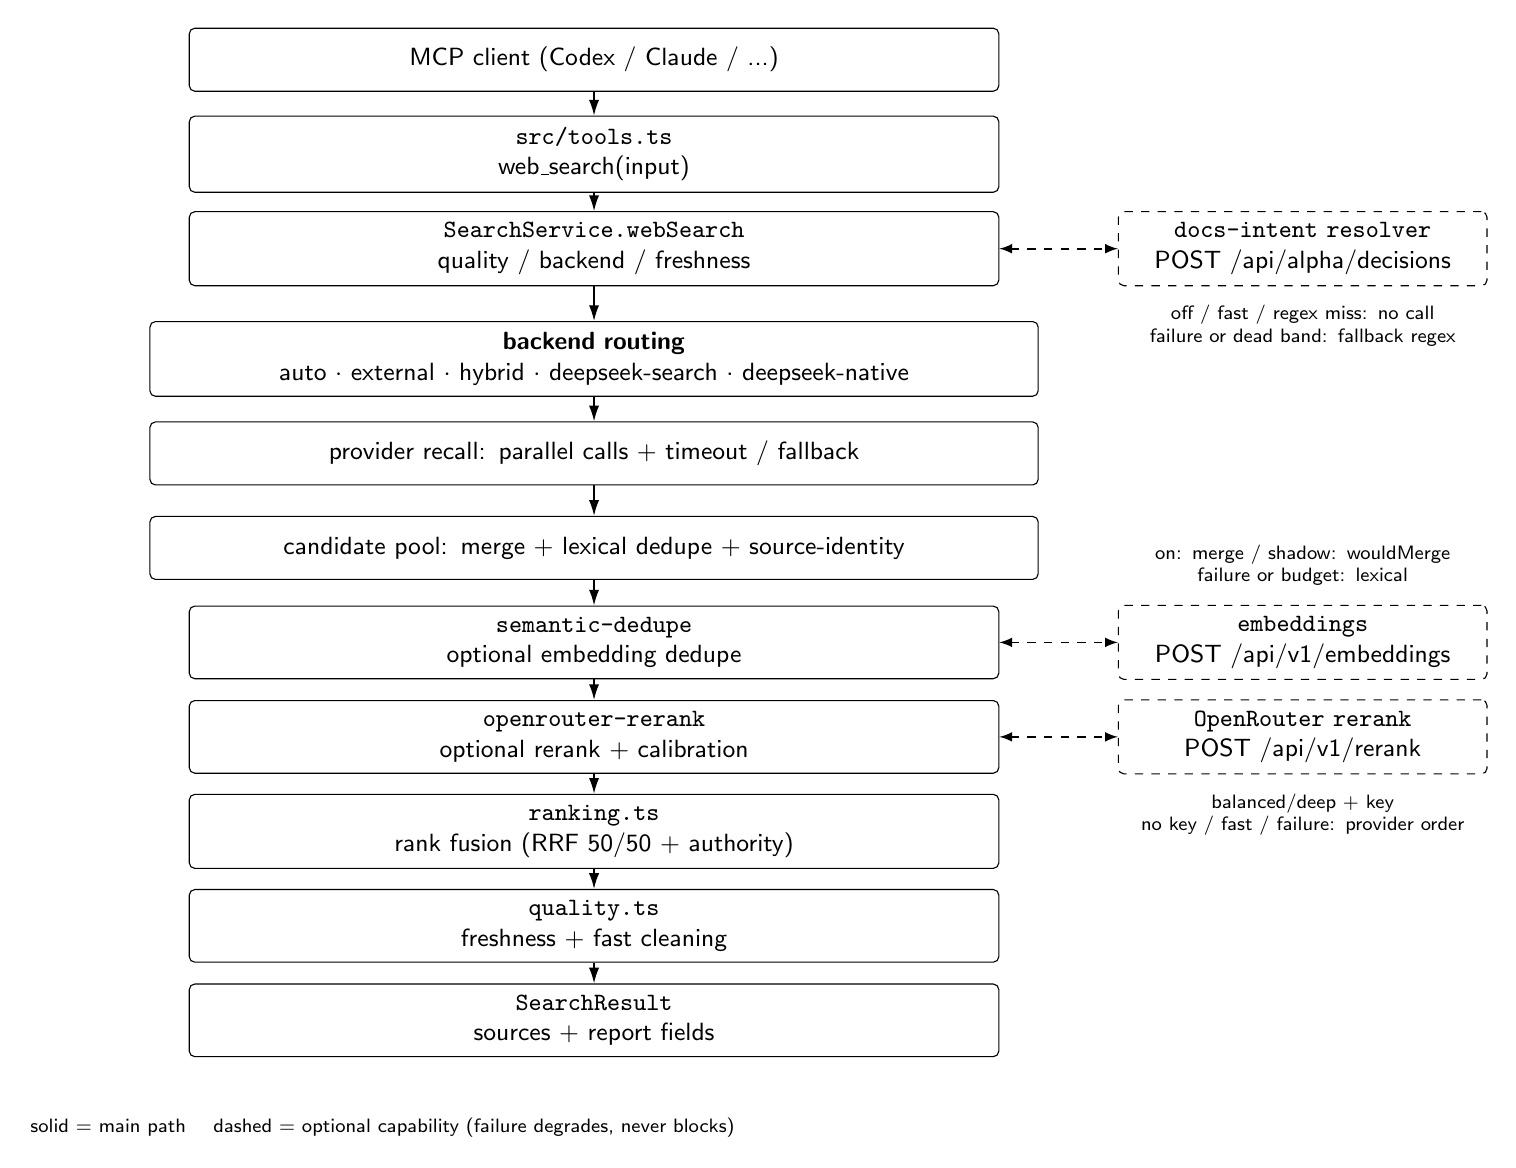
\begin{tikzpicture}

% main spine
\node[box] (client) at (0,10.6) {MCP client (Codex / Claude / ...)};
\node[box] (tools) at (0,9.4) {\texttt{src/tools.ts}\\web\_search(input)};
\node[box] (svc) at (0,8.2) {\texttt{SearchService.webSearch}\\quality / backend / freshness};
\node[box, text width=110mm] (routing) at (0,6.8) {\textbf{backend routing}\\auto $\cdot$ external $\cdot$ hybrid $\cdot$ deepseek-search $\cdot$ deepseek-native};
\node[box, text width=110mm] (providers) at (0,5.6) {provider recall: parallel calls + timeout / fallback};
\node[box, text width=110mm] (pool) at (0,4.4) {candidate pool: merge + lexical dedupe + source-identity};
\node[box] (sem) at (0,3.2) {\texttt{semantic-dedupe}\\optional embedding dedupe};
\node[box] (rer) at (0,2.0) {\texttt{openrouter-rerank}\\optional rerank + calibration};
\node[box] (fuse) at (0,0.8) {\texttt{ranking.ts}\\rank fusion (RRF 50/50 + authority)};
\node[box] (qual) at (0,-0.4) {\texttt{quality.ts}\\freshness + fast cleaning};
\node[box] (result) at (0,-1.6) {\texttt{SearchResult}\\sources + report fields};

\draw[arrow] (client) -- (tools);
\draw[arrow] (tools) -- (svc);
\draw[arrow] (svc) -- (routing);
\draw[arrow] (routing) -- (providers);
\draw[arrow] (providers) -- (pool);
\draw[arrow] (pool) -- (sem);
\draw[arrow] (sem) -- (rer);
\draw[arrow] (rer) -- (fuse);
\draw[arrow] (fuse) -- (qual);
\draw[arrow] (qual) -- (result);

% optional branches on the right
\node[branch] (dec) at (9.0,8.2) {\texttt{docs-intent resolver}\\POST /api/alpha/decisions};
\node[note, below=2mm of dec] (decnote) {off / fast / regex miss: no call\\failure or dead band: fallback regex};

\node[branch] (emb) at (9.0,3.2) {\texttt{embeddings}\\POST /api/v1/embeddings};
\node[note, above=2mm of emb] (embnote) {on: merge / shadow: wouldMerge\\failure or budget: lexical};

\node[branch] (rerank) at (9.0,2.0) {\texttt{OpenRouter rerank}\\POST /api/v1/rerank};
\node[note, below=2mm of rerank] (rernote) {balanced/deep + key\\no key / fast / failure: provider order};

\draw[ddbl] (svc.east) -- (dec.west);
\draw[ddbl] (sem.east) -- (emb.west);
\draw[ddbl] (rer.east) -- (rerank.west);

% legend
\node[lbl, anchor=north west, fill=none] at (-7.2,-2.8)
  {solid = main path \quad dashed = optional capability (failure degrades, never blocks)};

\end{tikzpicture}
\end{document}